\documentclass{SGGW-thesis}

\INZYNIERSKAtrue
\WZIMtrue

\title{Zastosowanie metod uczenia maszynowego do stworzenia sztucznej inteligencji w turowych grach RPG}
\Etitle{The use of machine learning methods to create artificial intelligence in turn-based RPG games}
\author{Rafał Kuligowski}
\date{2023}
\album{205835}
\thesis{Praca dyplomowa na kierunku:}
\course{Informatyka}
\promotor{dra Marka Karwańskiego}
\pworkplace{Instytut Informatyki Technicznej\\Katedra Zastosowań Matematyki}

\usepackage[bottom]{footmisc}
\usepackage{hyperref}
\usepackage{subfigure}
\usepackage{float}

\begin{document}
\maketitle
\statementpage
\abstractpage
{Zastosowanie metod uczenia maszynowego do stworzenia sztucznej inteligencji w turowych grach RPG}
{Tematem pracy było implementowanie sztucznej inteligencji uczącej się za pomocą metod uczenia maszynowego w turowej grze RPG. Praca składa się z czterech głównych części.
Pierwsza część omawia technologie wykorzystane w pracy oraz ich alternatywy. Druga część skupia się na implementacji wcześniej wspomnianych technologii.
Trzecia część zawiera instrukcję użytkowania gotowej aplikacji. W czwartej części znajdują się wnioski dotyczące implementacji tematycznego rozwiązania w szerszym kontekście.}
{uczenie maszynowe, sztuczna inteligencja, gry RPG, uczenie przez wzmacnianie, turowe systemy walki}
{The use of machine learning methods to create artificial intelligence in turn-based RPG games}
{The topic of the paper was the implementation of artificial intelligence, which learns through machine learning methods, in a turn-based RPG game. 
The paper consists of four main parts. The first part discusses the technologies used in the work and their alternatives. The second part focuses on 
the implementation of the aforementioned technologies. The third part contains user instructions for the finished application. The fourth part includes 
conclusions regarding the implementation of the thematic solution in a broader context.}
{machine learning, artificial intelligence, RPG games, reinforcement learning, turn-based battle system}


{
  % Spis treści może być złożony z pojedynczą interlinią, np. jeśli jedna linia wychodzi na następną stronę.
  % W przeciwnym razie spis treści wstawić bez powyższego rozkazu i klamry.
  \doublespacing
  \tableofcontents
}

\startchapterfromoddpage % niezależnie od długości spisu treści pierwszy rozdział zacznie się na nieparzystej stronie

\chapter{Wstęp}
Sztuczna Inteligencja w przeciągu ostatnich lat objęła wiele dziedzin życia i jest ciągle dynamicznie rozwijana. Jej zastosowanie jest bardzo 
rozległe, a jedną z branż o dużych perspektywach rozwoju tej technologii jest przemysł rozrywkowy w który wchodzą gry wideo. W grach można zastosować 
tą technologię do chociażby generowania misji i zadań dla graczy aby nie były one powtarzalne, stworzenia mądrego systemu automatycznej walki dzięki
któremu gracz nie lubiący tego elementu w grze może go pominąć, czy też do stworzenia sztucznej inteligencji dla przeciwników gracza. Ostatnie z tych 
przykładowych zastosowań zostanie zgodnie z tematem pracy omówione pod względem teoretycznym i praktycznym.


\section{Cel i zakres pracy}
Praca ma na celu zbadanie możliwości implementacji sztucznej inteligencji dla przeciwnków w grach wideo z gatunku RPG\footnote{RPG (ang. Role Playing Games) 
- gry w których gracz wciela się w rolę postaci występujących w fikcyjnym świecie. Gracze ponoszą wszelkie konsekwencje swoich akcji jako postać w świecie gry.}
z turowym systemem walki. Wynikowo otrzymamy 2 aplikacje: trenującą model oraz testującą model w postaci symulatora walki. Treść pracy będą stanowić opisy technologii
użytych w pracy wraz z alternatywami, opis implementacji rozwiązania na podstawie wybranych wcześniej technologii, instrukcję obsługi napisanej aplikacji oraz
wnioski na temat implementacji takiego rozwiązania w szerszym zakresie.


\chapter{Technologie}
W tym rozdziale zostaną szczegółowo omówione komponenty potrzebne do implementacji takowej sztucznej inteligencji. Według kolejności wyboru są to: 
\begin{itemize}
  \item{Rodzaj uczenia maszynowego}
  \item{Silnik do stworzenia gry oraz pakiet do uczenia maszynowego kompatybilny z silnikiem}
  \item{Wykorzystywany algorytm do uczenia maszynowego}
  \item{System walki (w przypadku tej pracy - system oparty o tury)}
\end{itemize}


\section{Rodzaje uczenia maszynowego}
W uczeniu maszynowym można rozgraniczyć 3 jego główne rodzaje (w oparciu o drugi rozdział z~\cite{MachineLearningTypes}):
\begin{itemize}
  \item{Nadzorowane (ang. Supervised) - model jest trenowany na danych wejściowych oraz odpowiednich dla nich wartości wynikowych. Na ich podstawie uczy się przewidywania wyniku dla nowych, nieznanych danych wejściowych.}
  \item{Nienadzorowane (ang. Unsupervised) - model jest trenowany na samych danych wejściowych nie dostając oczekiwanych wyników. Model sam musi odkryć sens jaki stoi za danymi wejściowymi.}
  \item{Przez wzmacnianie (ang. Reinforcement) - model trenowany za pomocą interakcji trenowanego agenta z wykreowanym otoczeniem. Agent wykonując akcje w otoczeniu dostaje nagrody lub kary w zależności od wyników jego akcji.}
\end{itemize}
W przypadku tej pracy użyty zostanie rodzaj uczenia przez wzmacnianie przez charakterystyczną dla niego metodę uczenia przez interakcje. Metoda ta pasuje do gier wideo, gdyż z założenia polegają one na interakcji gracza ze światem gry.
Model będzie mógł, tak samo jak gracz grający w grę, poprzez ingerowanie za pomocą akcji w otoczenie uczyć się wykonywania najlepszych możliwych akcji w danym momencie. Wiecej wiedzy o tym jak działa uczenie przez wzmacnianie jest zawarte w~\cite{ReinforcementLearning}.


\section{Silniki graficzne oraz pakiety do uczenia}
Wybór silnika graficznego oraz pakietu do uczenia maszynowego jest ze sobą głęboko powiązany. Ponadto jest on mocno subiektywny, gdyż jest uzależniony od umiejętności autora projektu. Lista popularnych wyborów w zakresie silnika i pakietu do uczenia maszynowego:
\subsection{Unity z pakietem ML-Agents}
Wśród wymienionych gotowych pakietów, ML-Agents jest najstarszym rozwiązaniem (udostępnione w 2017r.\footnote{Repozytorium powstało 8.09.2017r, pierwsza wersja pakietu pochodzi z 16.09.2017r - link do repozytorium \url{https://github.com/Unity-Technologies/ml-agents}}).
Dostępne w pakiecie są 2 algorytmy uczenia przez wzmacnianie - PPO oraz SAC\footnote{Więcej informacji o tych algorytmach w rozdziale "\nameref{algorithms}"}. Pakiet posiada własną dokumentację\cite{MLAgentsDocs}. 
Sam silnik Unity umożliwia tworzenie aplikacji z grafiką 2D oraz 3D, operuje na łatwym w nauce języku C\# oraz ma rozbudowaną dokumentację\cite{UnityDocs}.
\subsection{Godot z pakietem RL Agents}
Godot jest silnikiem OpenSource o coraz mocniejszej pozycji na rynku. Według dokumentacji\cite{GodotDocs}
silnik wspiera oficjalnie 2 języki programowania: autorski język GDScript oraz C\#. Twórcy za pośrednictwem technologii GDExtension dodali możliwość dodania wsparcia dla innych języków przez społeczność.
Dzięki temu, można na tym silniku programować również w innych językach programowania takimi jak Rust, C++ czy Swift. Pakiet RL Agents jest najbardziej rozbudowanym pakietem wśród wymienionych.
Bazuje na 4 innych pakietach\footnote{Pakiety na których bazuje RL Agents - StableBaseLines3, SampleFactory, CleanRL oraz Ray rllib (stan na 06.01.2024r.)} do uczenia przez wzmacnianie
oraz wspiera ponad 12 algorytmów uczenia. Więcej informacji o RL Agents można znaleźć w artykule naukowym poświęconym tej technologii~\cite{GodotRLAgentsArticle} oraz w dokumentacji dostępnej w repozytorium projektu~\cite{GodotRLAgentsDocs}.
\subsection{Unreal Engine z pakietem Learning Agents}
Pod względen innych pakietów Learning Agents jest najmłodszy (powstał na początku 2023r.) oraz najsłabiej udokumentowany. Pakiet operuje algorytmami PPO oraz BC (ang. Behavioral Cloning) \footnote{Informacja pochodzi ze źródła (stan na 06.01.2024r.): \url{https://dev.epicgames.com/community/learning/tutorials/8OWY/unreal-engine-learning-agents-introduction}}. 
Mimo to sam silnik Unreal Engine jest potężnym narzędziem z bardzo dużym wsparciem i możliwościami. Posiada wsparcie dla języka C++ oraz funkcji Blueprints umożliwiającej programowanie wizualne (bez pisania kodu). 
Dokumentacja zarówno silnika Unreal Engine jak i pakietu Learning Agents znajduje się w~\cite{UnrealDocs}.
\subsection{Własny silnik z wykorzystaniem różnych pakietów do uczenia maszynowego}
Rozwiązanie oferujące największą swobodę, ale też najtrudniejsze w implementacji. Do stworzenia środowiska gry potrzebna jest biblioteka graficzna pomagająca stworzyć silnik np. OpenGL
lub pakiet do stworzenia aplikacji okienkowej np. PyGame. Wybierając pakiet do uczenia maszynowego warto szukać wśród pakietów Pythona gdyż ma on ich bardzo dużo. Dla uczenia przez wzmocnienie można zastosować pakiet PyTorch\footnote{Używany w ML-Agents oraz Learning Agents}
lub też jeden z 4 pakietów wykorzystywanych przez RL Agents.
\subsection*{Wybrany silnik i pakiet do uczenia maszynowego}
Do pracy wybrałem Unity z pakietem ML-Agents przez moje wcześniejsze doświadczenie z Unity oraz zaawansowanie w języku C\#. Uważam jednak, że dużo bardziej rozbudowany RL Agents na silniku Godot jest lepszym wyborem do tego typu projektu, gdyż daje dużo większe pole do dostosowania uczenia dla osiągnięcia lepszych rezultatów.


\section{Algorytmy do uczenia maszynowego}
\label{algorithms}
Unity ML-Agents posiada 2 algorytmy uczące PPO (ang. Proximal Policy Optimization) oraz SAC (ang. Soft Actor-Critic). Pierwszy z nich jest podstawowym algorytmem używanym w pakiecie. Według \cite{MLAgentsDocs} algorytm PPO jest algorytmem ogólnego przeznaczenia i jest bardziej stabilny w porównaniu z innymi algorytmami uczenia przez wzmacnianie.
To samo źródło opisuje również różnicę między algorytmem SAC i PPO. SAC jest algorytmem "off-policy" kiedy PPO jest algorytmem "on-policy". Oznacza to że SAC uczy się z doświadczeń zebranych w dowolnym momencie w przeszłości, a podczas uczenia są losowo dobierane do treningu, gdzie w PPO występuje "policy",
które reguluje podejmowanie decyzji i jest ulepszane z każdą iteracją uczenia. Dodatkowe informacje o algorytmie PPO znajdują się w~\cite{PPOArticle}, a o SAC w~\cite{SACArticle}. Do projektu wybrany został algorytm PPO z uwagi na wcześniej podaną stabilność oraz fakt, że jest on algorytmem będącym ponad 6 lat w pakiecie ML-Agents co sugeruje, że jest on lepiej rozwiniętym rozwiązaniem w pakiecie.

\section{Systemy walki w turowych grach RPG}
Systemów walki turowej w grach RPG jest bardzo dużo, ale wszystkie charakteryzują się paroma wspólnymi cechami:
\begin{itemize}
  \item{Rozgrywka polega na wymianie tur postaci gracza z przeciwnikami}
  \item{Podczas tury gracz oraz przeciwnicy wykorzystują swoje tury jako zasób do wykonywania akcji}
  \item{Postacie gracza oraz przeciwnicy posiadają statystyki, które określają ich cechy. Do takich statystyk może należeć np. Obrona zmniejszająca obrażenia otrzymywane przez postać, czy też Atak zwiększający zadawane obrażenia}
  \item{Postacie gracza oraz przeciwnicy posiadają umiejętności, których mogą używać zużywając tury do wykonywania akcji w środowisku gry}
  \item{Walka kończy się gdy wszystkie postacie gracza lub wszyscy przeciwnicy umrą}
\end{itemize}
Poniżej przedstawię parę podejść do turowego systemu walki wraz z przykładową grą w której został taki system walki użyty:
\subsection{Standart Turn Battle}
Najbardziej podstawowy, najpowszechniejszy i zarazem najprostszy system walki turowej. Na początku walki jest tworzona kolejka tur złożona ze wszystkich postaci na scenie na podstawie statystyki Szybkości.
Gdy postać wykorzysta swoją turę jest przenoszona na koniec kolejki i następna postać w kolejce dostaje możliwość wykorzystania tury. Posiada on 2 główne warianty:
\begin{enumerate}
  \item{Postać posiadająca turę od razu po wybraniu ruchu go wykonuje i kolejka przechodzi do następnej osoby. Jest to system wykorzystywany np. w grach z serii Pokemon, czy też jako podstawowy system walki w kreatorze gier RPG o nazwie RPG Maker MV.}
  \item{Wszystkie postacie na początku wybierają ruch jakiego będą używać podczas aktualnego przejścia przez kolejkę. Po wybraniu walka trwa jedno całe przejście kolejki, aby po ruchu ostatniej postaci w kolejce znów poprosić o wybranie ruchu. Jest to rozwiązanie znane np. z gier z serii Etrian Odyssey.}
\end{enumerate}
\subsection{Active Turn Battle}
System walki charakteryzuje sie tym, że każda postać na początku zaczyna z pustym paskiem tury ładującym się w równych interwałach o wartość zależną od statystyki Szybkości. Im większa owa statystyka, tym szybciej tura jest ładowana.
Gdy tura jakiejś postaci zostanie w pełni naładowana, walka zatrzymuje się, a postacie z naładowaną turą wybierają akcję jaką mają wykonać. Następnie pasek tury jest ponownie ładowany. Gdy dobiegnie do końca postać wykona wybraną wcześniej akcję i resetuje ładowanie tury do wartości początkowej.
System ten jest znany z gier z serii Final Fantasy.
\subsection{Press Turn System}
Został stworzony i w głównej mierze jest używany w grach firmy Atlus począwszy od gry~\cite{SMT3}. System opiera się o zwiększenie znaczenia tury jako zasobu gdzie na początku gra oddziela fazę ruchu gracza i przeciwnika. Następnie tworzy kolejkę ruchów dla uczestnikow danej fazy na podstawie statystyki Szybkości.
Następne kroki jakie podejmuje system są zależne od wariantu tego systemu. 

\subsubsection{Wariant klasyczny}
Występujący w grach z serii Shin Megami Tensei począwszy od \cite{SMT3}. Ilość tur dla strony wykonującej ruchy jest liczona na podstawie ilości postaci po tej stronie. Każda akcja wykonana przez postać jest oceniana przez system i na podstawie oceny zmienia się ilość tur. W przypadku tego modelu musi występować system 
Elementów, które są przypisane do każdej umiejętności ofensywnej, oraz relacji postaci do Elementu. Elementem mogą być np. żywioły takie jak Ogień, Lód czy Wiatr, natomiast relacjami są skutki Elementu na postać, które potem edytują ilość tur. W grach z tej serii występuje 6 relacji do Elementów:
\begin{enumerate}
  \item{Normalna}
  \item{Słabość}
  \item{Odporność}
  \item{Niewrażliwość}
  \item{Odbicie}
  \item{Absorpcja}
\end{enumerate}
Jeśli postać trafi w słaby punkt przeciwnika nie traci całej tury, a tura jest "wciskana" (ang. Pressed). To samo dzieje się, gdy postać trafi cios krytyczny. "Wciśnięta" tura zachowuje się jak zwykła tura, ale nie może być wciśnięta ponownie. Tury można "wciskać" trafiając w słaby punkt przeciwnika oraz uderzając ciosami krytycznymi aż do momentu, w którym nie będziemy mieli dostępnych zwykłych tur.
Jeśli posiadamy zarówno zwykłą turę, jak i "wciśniętą" turę to akcja z normalną relacją do Elementu spowoduje zużycie "wciśniętej" tury. Inne typy relacji zmniejszają ilość tur o określoną ilość np. trafienie w Element z relacją Niewrażliwości może obniżyć ilość tur atakującego o 2 priorytetyzując tury "wciśnięte".
Jeśli postać postanowi nic nie robić podczas tury, jest ona "wciskana". Gdy stronie wykonującej akcje skończą się tury następuje zmiana stron dla które takie same zasady są zachowane. W przypadku gdy walka jest z silniejszą postacią (tzw. Bossem), która występuje sama system daje tej postaci dodatkową turę na start.

\subsubsection{Wariant uproszczony}
Występujący w grach z serii Persona począwszy od części trzeciej. W tym przypadku również musi występować system Elementów i relacji opisany jak w wersji klasycznej. Postacie mogą wykonać jedną akcję według kolejki określonej na początku fazy. Jeśli po użyciu umiejętności ofensywnej postać trafi w słaby punkt przeciwnika lub uderzy cios krytyczny,
nie traci ruchu i może użyć czegoś jeszcze raz, a przeciwnik dostaje status "Powalenia". Jeśli trafi się przeciwnika o tym statusie ciosem krytycznym lub w słaby punkt, nie dostaje się dodatkowego ruchu i rusza się kolejna osoba z drużyny. Status "Powalenia" znika gdy postać ma się ruszyć. W każdym innym przypadku ruch jest tracony i rusza się kolejna osoba. 
W grze Persona 5 dodano dodatkowo mechanikę Baton Pass, która umożliwia oddanie swojej tury po trafieniu krytycznym lub w słaby punkt innej osobie z drużyny. Jeśli kolejna osoba trafi cios krytyczny lub w słaby punkt może oddać swoją turę kolejnej osobie z drużyny wyłączając każdą osobę która korzystała z tej mechaniki wcześniej. Po wykonaniu akcji nie dającej dodatkowego ruchu, 
ruch dostaje następna postać.


\subsection*{Wybrany system walki}
Do implementacji został wybrany klasyczny wariant systemu Press Turn z gry \cite{SMT3}. Mimo swojego skomplikowania (co może spowodować dłuższy czas uczenia modelu) posiada on bardzo dużo ciekawych interakcji związanych z turami, które sztuczna inteligencja będzie mogła wykorzystać na swoją korzyść.


\chapter{Implementacja}
Aplikacja jest podzielona na 2 części: automatycznie trenującą model oraz testującą model w symulatorze walki.


\section{Część aplikacji testująca model}
Ta część aplikacji została zaimplementowana jako pierwsza w celu przygotowania systemu Press-Turn. Składa się z 3 scen Unity: MainMenu, CharacterCreator oraz BattleScene.

\subsection{Scena MainMenu}
Menu Główne składa się z 2 widoków: Panelu głównego oraz opcji. W panelu głównym są dostępne przyciski START, CONFIG oraz EXIT. START służy do uruchomienia kreatora postaci, CONFIG otwiera widok opcji, a EXIT służy do zamknięcia aplikacji\footnote{Przycisk zamknięcia aplikacji nie działa podczas testowania aplikacji na silniku, tylko gdy aplikacja zostanie wyeksportowana.}.
Widok opcji posiada suwaki zmieniające głośność muzyki oraz dźwięków w aplikacji i przycisk zapisujący ustawienia.

\begin{figure}[H]
  \hfill
  \subfigure[Widok panelu głównego]{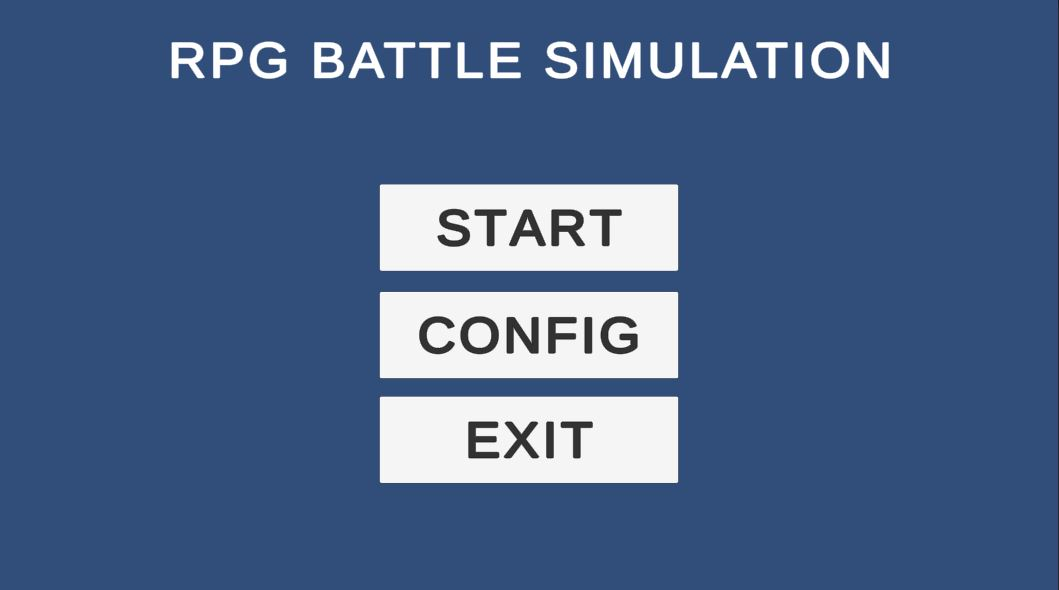
\includegraphics[width=0.45\textwidth]{menuscreen1.JPG}}
  \hfill
  \subfigure[Widok opcji]{
\includegraphics[width=0.45\textwidth]{menuscreen2.JPG}}
  \hfill
  \caption{Zrzuty ekranu przedstawiające menu główne}
\end{figure}

\subsection{Scena CharacterCreator}
Kreator postaci składa się z 2 widoków: panelu wyboru liczby aktorów w drużynie oraz kreatora postaci. Oba widoki posiadają też przycisk BACK powracający do menu głównego.


\subsubsection{Panel wyboru liczby aktorów}
Panel składa się z suwaka przyjmującego wartości całkowite w zakresie 1-4 oraz przycisk potwierdzający ilość aktorów o treści ACCEPT. Po jego wciśnięciu widok zmienia się na kreator postaci.

\subsubsection{Kreator postaci}
Składa się z przycisku Restart Actors wracającego do widoku wyboru liczby aktorów, przycisku Start Battle zaczynającego walkę gdy wszyscy aktorzy mają wypełnione pola statystyk, pola wyboru aktualnie edytowanego aktora oraz obszernego ekranu do wprowadzania statystyk postaci.
Lista statystyk postaci (sens statystyk zostanie wyjaśniony podczas omawiania sceny walki):
\begin{enumerate}
  \item{HP (ang. Health Points, pl. Punkty Życia) - zakres 1-9999}
  \item{MP (ang. Mana Points, pl. Punkty Many) - zakres 1-9999}
  \item{Strength (pl. Siła) - zakres 1-99}
  \item{Magic (pl. Magia) - zakres 1-99}
  \item{Dexterity (pl. Sprawność) - zakres 1-99}
  \item{Agility (pl. Zwinność) - zakres 1-99}
  \item{Luck (pl. Szczęście) - zakres 1-99}
\end{enumerate}
Postacie posiadają również Elementy i odpowiadające im relacje. Lista Elementów (kolejność od lewej według ustawienia w widoku):
\begin{enumerate}
  \item{Obrażenia fizyczne}
  \item{Ogień}
  \item{Lód}
  \item{Wiatr}
  \item{Elektryczność}
  \item{Światłość}
  \item{Ciemność}
  \item{Nadzwyczajny - ukryty element, zawsze o relacji neutralnej}
\end{enumerate}
Lista relacji Elementu z postacią (wraz ze skrótem widocznym w kreatorze, wpływem na tury oraz wpływem na obrażenia):
\begin{enumerate}
  \item{Neutralny, skrót: "-", wpływ na turę: utrata 1 tury, wpływ na obrażenia: brak}
  \item{Słabość, skrót: "Wk", wpływ na turę: "wciśnięcie" 1 tury, wpływ na obrażenia: +20\%}
  \item{Odporność, skrót: "Str", wpływ na turę: utrata 1 tury, wpływ na obrażenia: -20\%}
  \item{Niewrażliwość, skrót: "Null", wpływ na turę: utrata 2 tur, wpływ na obrażenia: zniwelowanie obrażeń}
  \item{Odbicie, skrót: "Rep", wpływ na turę: utrata 4 tur, wpływ na obrażenia: odbicie wartości obrażeń (obrażenia odbite również podlegają ocenie, ale nie wpływają na tury oraz nie mogą odbić się drugi raz)}
  \item{Absorbcja, skrót: "Abs", wpływ na turę: utrata 4 tur, wpływ na obrażenia: wyleczenie o wartość obrażeń}
\end{enumerate}
W skład kreatora wchodzi również lista z wyborem umiejętności. Każdy rekord listy posiada: pole wyboru umiejętności, jej nazwę, koszt oraz przypisany Element.

\begin{figure}[H]
  \hfill
  \subfigure[Widok panelu wyboru liczby aktorów]{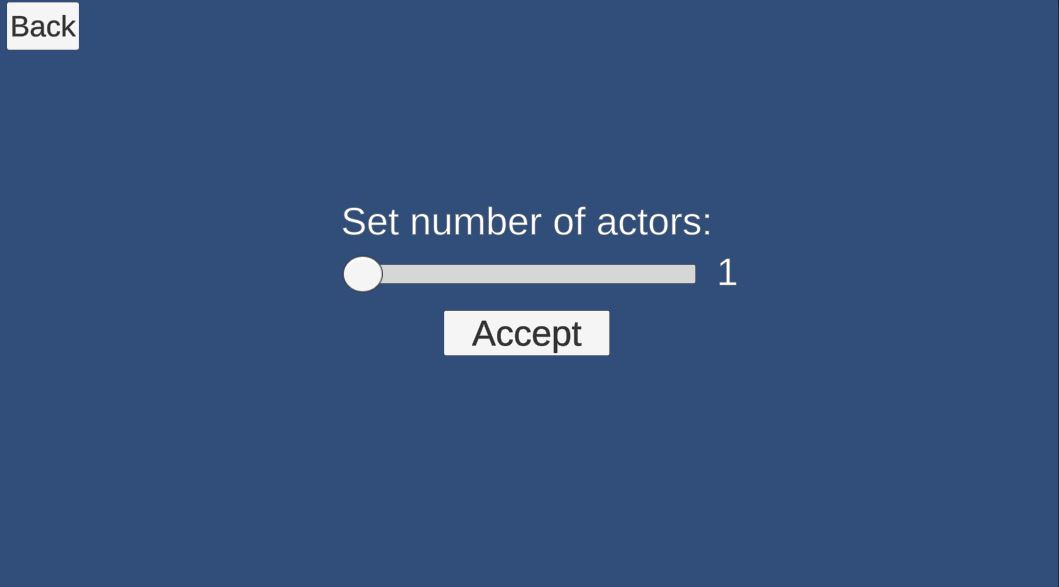
\includegraphics[width=0.45\textwidth]{creatorscreen1.JPG}}
  \hfill
  \subfigure[Widok kreatora postaci]{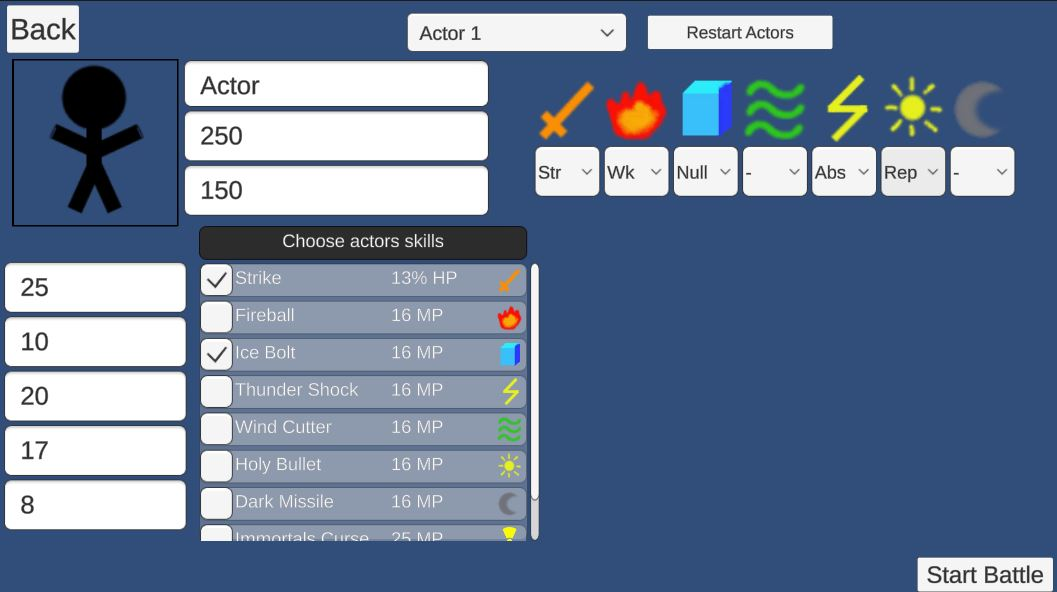
\includegraphics[width=0.45\textwidth]{creatorscreen2.JPG}}
  \hfill
  \caption{Zrzuty ekranu przedstawiające kreator postaci}
\end{figure}

\subsection{Scena BattleScene}
Rozbudowana scena przedstawiająca informacje na temat aktualnego stanu walki. Stworzona na podstawie UI z gry~\cite{SMT3}.

Scena posiada następujące elementy UI:
\begin{itemize}
  \item{Przycisk Leave Battle - służy do wyjścia z walki}
  \item{Lista tur - czerwone znaczniki oznaczają "wciśnięte" tury, a zielone zwykłe tury}
  \item{Widok drużyny gracza - generowany automatycznie, obramowanie pokazuje kto aktualnie posiada ruch}
  \item{Widok przeciwnika - sterowany przez wytrenowany model przeciwnik z widocznym paskiem zdrowia}
  \item{Lista umiejętności - umożliwia wybór umiejętności aktualnie ruszającej się postaci. Po wyborze umiejętności gracz jest proszony o cel.}
  \item{Dziennik zdarzeń walki - pokazuje umiejętności użyte od początku walki przez jakąkolwiek postać}
  \item{Stan drużyny gracza - pokazuje paski z imionami wszystkich postaci gracza, jak i ich stanem zdrowia i many}
\end{itemize}

\begin{figure}[H]
  \hfill
  \subfigure[UI gry~\cite{SMT3}]{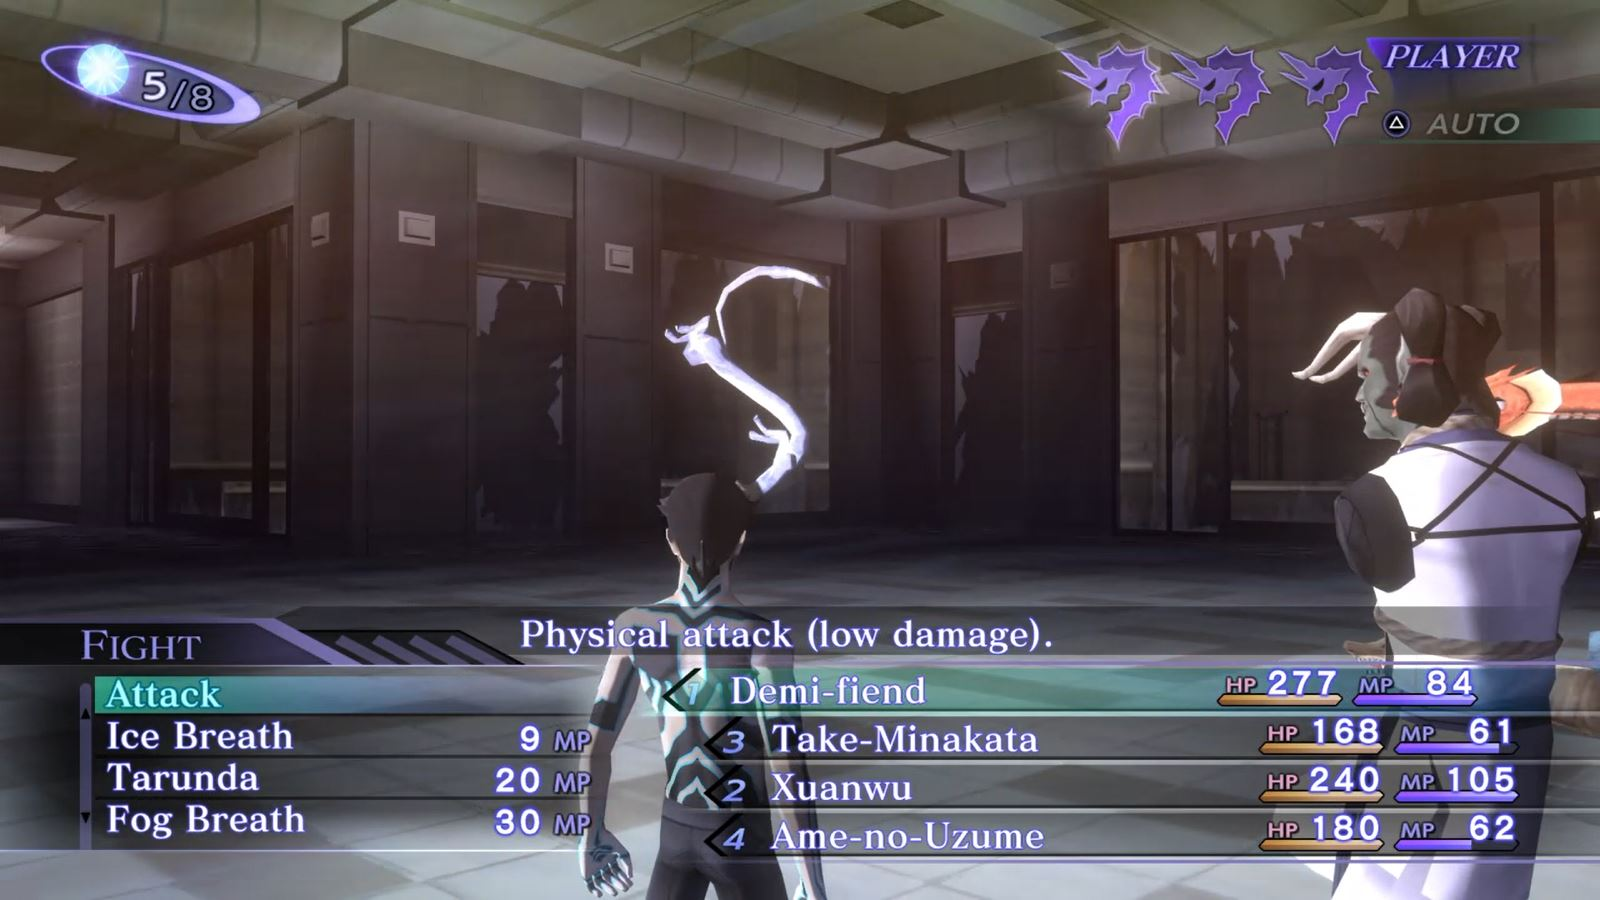
\includegraphics[width=0.45\textwidth]{smt3_screenshot.jpg}}
  \hfill
  \subfigure[UI sceny walki w projekcie]{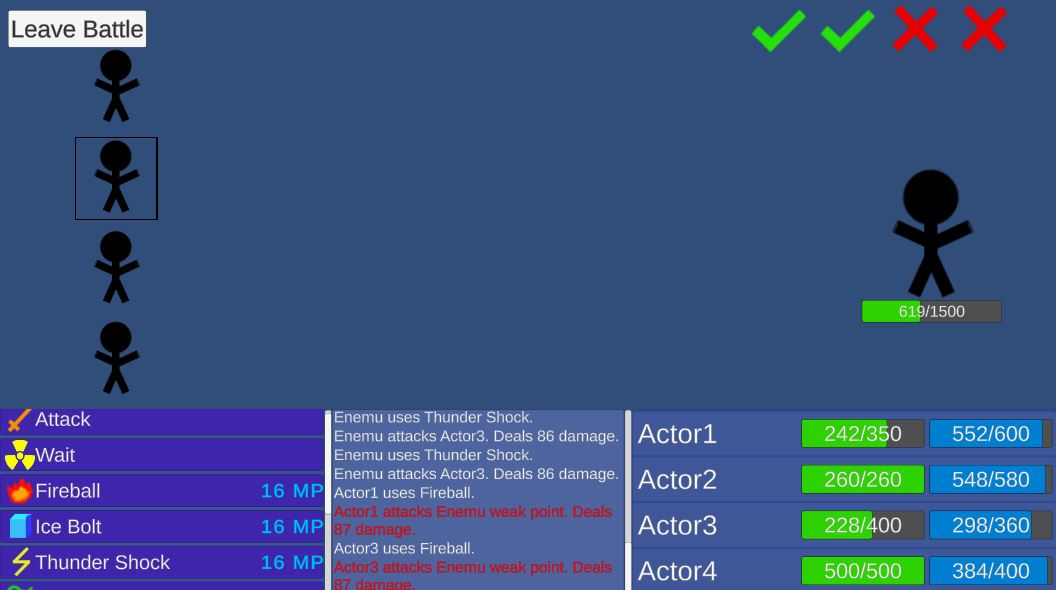
\includegraphics[width=0.45\textwidth]{battlescreen.JPG}}
  \hfill
  \caption{Zrzuty ekranu porównujące UI stworzone w projekcie do występującego w grze \cite{SMT3}}
\end{figure}

\subsection{Implementacja systemu Press Turn}
System Press Turn zaimplementowany w projekcie działa na 2 obiektach:
\begin{itemize}
  \item{BattleManager - odpowiada za logikę walki}
  \item{BattleData - przechowuje dane o postaciach, stanach i umiejętnościach}
\end{itemize}
Zanim wczyta się scena BattleScene, w kreatorze jest tworzony obiekt BattleData. Przed wypełnieniem go danymi o postaciach posiada informacje o stanach, 
jakich postacie mogą doznać (aktualnie zaimplementowany jest tylko stan Śmierci), oraz spis wszystkich umiejętności. Obiekt jest wypełniany danymi z
kreatora dotyczącymi postaci. Dane te są zapisywane do dwóch list:
\begin{itemize}
  \item{party - przechowująca postaci sterowane przez gracza}
  \item{enemies - przechowująca informacje o postaci przeciwnika}
\end{itemize}
Po wczytaniu się sceny, BattleManager zostaje zainicjowany. Posiada on następujące wartości:
\begin{itemize}
  \item{selectedSkill - przechowuje informacje na temat wybranej przez postać umiejętności}
  \item{isPlayerTurn - wartość prawda/fałsz mówiąca czy rusza się gracz, bazowo ustawiony na prawdę}
  \item{isBusy - wartość prawda/fałsz odpowiadająca za przejście do następnego stadium walki, bazowo ustawiony na prawdę}
  \item{gameState - enumerator mówiący jakie jest stadium walki, może przyjąć jedną z następujących wartości: START\_SIDE, START\_TURN, END\_SIDE, END\_TURN}
  \item{currentCharacter - przechowuje informacje o aktualnie poruszającej się postaci}
  \item{moveQueue - lista z indeksami postaci ułożona w kolejności poruszania się (sortowana po statystyce Agility, od największej wartości do najmniejszej)}
  \item{currentIndex - wartość pomocnicza przechowująca indeks aktualnie poruszającej się postaci}
  \item{turnQueue - lista z wartościami prawda fałsz odpowiadająca ilości tur (zwykłe tury to wartości true, "wciśnięte" tury to wartości false)}
\end{itemize}

\subsubsection{Główna pętla systemu walki}
Po wczytaniu wszystkich potrzebnych zasobów, BattleManager ustawia wartości gameState na START\_SIDE oraz isBusy na false. Sam system walki operuje na funkcji Update wykonującej się co klatkę. Dokoładniejszy opis działania funkcji Update można znaleźć w~\cite{UnityDocs}. 
\begin{figure}[H]
  \centering
  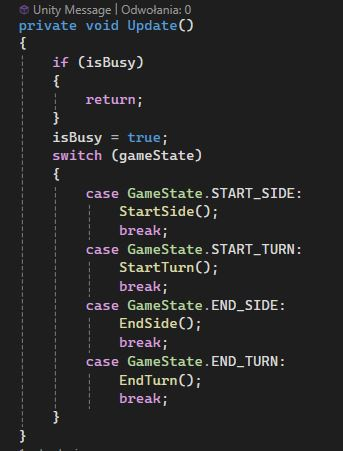
\includegraphics[height=7cm]{updatebattle.JPG}
  \caption{Funkcja Update w obiekcie BattleManager}
  \label{fig:UpdateBattle}
\end{figure}

Cała pętla gry operuje na wywoływaniu 4 funkcji podanych na \hyperref[fig:UpdateBattle]{Rysunek 3.4}. Przedstawiona w postaci listy kroków prezentuje się następująco:
\begin{enumerate}
  \item{Wywołuje się StartSide(), które uzupełnia listę tur - turnQueue oraz listę indeksów postaci - moveQueue}
  \item{Następuje aktualizacja currentIndex o pierwszy indeks z moveQueue, przenosząc ten index później na koniec listy moveQueue. Potem zmienia gameState na START\_TURN}
  \item{Wywołuje się StartTurn(), które ustawia wartość currentCharacter na aktualnie poruszającą się postać.}
  \item{Jeśli ruch wykonuje gracz aplikacja pokazuje dostępne umiejętności postaci i czeka na reakcję użytkownika}
  \item{Jeśli ruch wykonuje przeciwnik uruchamiana jest funkcja AIActions() która prosi o podjęcie decyzji wytrenowany model ML-Agents w wyborze celu oraz umiejętności}
  \item{Po wyborze umiejętności i celu wykonuje się funkcja UseSkill() uruchamiająca logikę systemu Press Turn}
  \item{Na koniec gameState jest zmieniany na END\_TURN}
  \item{Wywołuje się EndTurn(), które sprawdza warunki wygranej i przegranej (jeśli któryś z warunków jest prawdziwy, przejdź do 11.)}
  \item{Jeśli turnQueue jest puste, zmień stan na END\_SIDE, w przeciwnym wypadku przejdź do punktu 2.}
  \item{Wywołaj funkcję END\_SIDE, któa zmienia wartość isPlayerTurn na przeciwną sobie i zmienia wartość gameState na START\_SIDE. Przejdź do punktu 1.}
  \item{Pokaż ekran końcowy i opuść pętlę gry}
\end{enumerate}

\subsubsection{Funkcja UseSkill() oraz wykorzystanie statystyk}
Głównym zadaniem funkcji jest pobranie zasobów (many oraz zdrowia) potrzebnych do użycia wybranej umiejętności, aktywacja tejże umiejętności na wybranym celu oraz zmiana tur na podstawie wyniku aktywacji.
Gdy dochodzi do aktywacji umiejętności, statystyki postaci atakującej i broniącej są przekazywane do funkcji przeliczającej obrażenia. Formuły obrażeń prezentują się nastepująco:
\[PhysicalAttack = 5*\sqrt{\frac{a.Strength}{b.Dexterity}*m}\]\[MagicalAttack = 5*\sqrt{\frac{a.Magic}{b.Dexterity}*m}\]
gdzie,
\begin{itemize}
  \item{a - atakujący}
  \item{b - broniący}
  \item{m - stała moc umiejętności}
\end{itemize}
Jedyna niewykorzystywana nigdzie statystyka to Luck, z uwagi na brak planowanej wcześniej implementacji ciosów krytycznych w systemie walki.


\section{Część aplikacji automatycznie trenująca model}
Ta część aplikacji służy do uczenia modelu, jak poruszać się po systemie Press Turn. Składa się z 1 sceny Unity: TrainingScene.


\subsection{Implementacja ML-Agents}


\subsection{UI}


\chapter{Instrukcja instalacji i korzystania}


\chapter{Wnioski}

\begin{thebibliography}{9}
  \bibitem{MachineLearningTypes}
  Shagan Sah,
  \textit{Machine Learning: A Review of Learning Types},
  (2020 r.)

  \bibitem{ReinforcementLearning}
  Vincent François-Lavet, Peter Henderson, Riashat Islam, Marc G. Bellemare, Joelle Pineau,
  \textit{An Introduction to Deep Reinforcement Learning},
  (2018 r.)

  \bibitem{MLAgentsDocs}
  \textit{Unity ML-Agents Toolkit Documentation} 
  \url{https://unity-technologies.github.io/ml-agents/ML-Agents-Toolkit-Documentation/}
  (dostęp 06.01.2024r)

  \bibitem{UnityDocs}
  \textit{Unity Documentation}
  \url{https://docs.unity.com}
  (dostęp 06.01.2024r)

  \bibitem{GodotDocs}
  \textit{Godot Documentation}
  \url{https://docs.godotengine.org/en/stable}
  (dostęp 06.01.2024r)

  \bibitem{GodotRLAgentsArticle}
  Edward Beeching, Jilles Debangoye, Olivier Simonin, Christian Wolf,
  \textit{Godot Reinforcement Learning Agents},
  (2021 r.)

  \bibitem{GodotRLAgentsDocs}
  \textit{Godot RL Agent Repository}
  \url{https://github.com/edbeeching/godot_rl_agents}
  (dostęp 06.01.2024r)

  \bibitem{UnrealDocs}
  \textit{Unreal Engine Documentation}
  \url{https://docs.unrealengine.com}
  (dostęp 06.01.2024r)
  
  \bibitem{PPOArticle}
  John Schulman, Filip Wolski, Prafulla Dhariwal, Alec Radford, Oleg Klimov, 
  \textit{Proximal Policy Optimization Algorithms},
  (2017 r.)

  \bibitem{SACArticle}
  Tuomas Haarnoja, Aurick Zhou, Pieter Abbeel, Sergey Levine, 
  \textit{Soft Actor-Critic: Off-Policy Maximum Entropy Deep Reinforcement Learning with a Stochastic Actor},
  (2018 r.)

  \bibitem{SMT3}
  Atlus,
  \textit{Shin Megami Tensei III},
  (2003 r.)
\end{thebibliography}

\beforelastpage

\end{document}